\IfFileExists{stacks-project.cls}{%
\documentclass{stacks-project}
}{%
\documentclass{amsart}
}
\usepackage{amssymb}

% For dealing with references we use the comment environment
\usepackage{verbatim}
\usepackage{fancyvrb}
\newenvironment{reference}{\comment}{\endcomment}
%\newenvironment{reference}{}{}
\newenvironment{slogan}{\comment}{\endcomment}
\newenvironment{history}{\comment}{\endcomment}

% For source figures retained as assets
\usepackage{graphicx}

% For commutative diagrams we use Xy-pic
\usepackage[all]{xy}

% We use 2cell for 2-commutative diagrams.
\xyoption{2cell}
\UseAllTwocells

% We use multicol for the list of chapters between chapters
\usepackage{multicol}

% This is generally recommended for better output
\usepackage{lmodern}
\usepackage[T1]{fontenc}
\usepackage{textalpha}

% For cross-file-references
% We prefer the snapshot tmp/xref/#2.aux,
% which latexmkrc replaces atomically, so
% that documents compiled simultaneously
% never read a half-written .aux file.
% The last argument keeps links to #2.pdf.
\usepackage{xr-hyper}
\newcommand{\maybeexternaldocument}[2]{%
  \IfFileExists{#2.aux}{%
    \externaldocument[#1]{#2}%
  }{%
    \PackageWarning{stack}{Missing #2.aux; external references with prefix #1 unavailable}%
  }%
}
\let\externaldocumentorig\externaldocument
\renewcommand{\externaldocument}[2][]{%
  \IfFileExists{tmp/xref/#2.aux}{%
    \externaldocumentorig[#1]{tmp/xref/#2}[#2.pdf]%
  }{%
  \IfFileExists{#2.aux}{%
    \externaldocumentorig[#1]{#2}%
  }{%
    \PackageWarning{stack}{Missing #2.aux; external references with prefix #1 unavailable}%
  }%
  }%
}

% Package for hypertext links:
\usepackage{hyperref}

% For any local file, say "hello.tex" you want to link to please
% use \externaldocument[hello-]{hello}
\externaldocument[introduction-]{introduction}
\externaldocument[conventions-]{conventions}
\externaldocument[sets-]{sets}
\externaldocument[categories-]{categories}
\externaldocument[topology-]{topology}
\externaldocument[sheaves-]{sheaves}
\externaldocument[sites-]{sites}
\externaldocument[stacks-]{stacks}
\externaldocument[fields-]{fields}
\externaldocument[algebra-]{algebra}
\externaldocument[brauer-]{brauer}
\externaldocument[homology-]{homology}
\externaldocument[derived-]{derived}
\externaldocument[simplicial-]{simplicial}
\externaldocument[more-algebra-]{more-algebra}
\externaldocument[smoothing-]{smoothing}
\externaldocument[modules-]{modules}
\externaldocument[sites-modules-]{sites-modules}
\externaldocument[injectives-]{injectives}
\externaldocument[cohomology-]{cohomology}
\externaldocument[sites-cohomology-]{sites-cohomology}
\externaldocument[dga-]{dga}
\externaldocument[dpa-]{dpa}
\externaldocument[sdga-]{sdga}
\externaldocument[hypercovering-]{hypercovering}
\externaldocument[schemes-]{schemes}
\externaldocument[constructions-]{constructions}
\externaldocument[properties-]{properties}
\externaldocument[morphisms-]{morphisms}
\externaldocument[coherent-]{coherent}
\externaldocument[divisors-]{divisors}
\externaldocument[limits-]{limits}
\externaldocument[varieties-]{varieties}
\externaldocument[topologies-]{topologies}
\externaldocument[descent-]{descent}
\externaldocument[perfect-]{perfect}
\externaldocument[more-morphisms-]{more-morphisms}
\externaldocument[flat-]{flat}
\externaldocument[groupoids-]{groupoids}
\externaldocument[more-groupoids-]{more-groupoids}
\externaldocument[etale-]{etale}
\externaldocument[chow-]{chow}
\externaldocument[intersection-]{intersection}
\externaldocument[pic-]{pic}
\externaldocument[weil-]{weil}
\externaldocument[adequate-]{adequate}
\externaldocument[dualizing-]{dualizing}
\externaldocument[duality-]{duality}
\externaldocument[discriminant-]{discriminant}
\externaldocument[derham-]{derham}
\externaldocument[local-cohomology-]{local-cohomology}
\externaldocument[algebraization-]{algebraization}
\externaldocument[curves-]{curves}
\externaldocument[resolve-]{resolve}
\externaldocument[models-]{models}
\externaldocument[functors-]{functors}
\externaldocument[equiv-]{equiv}
\externaldocument[pione-]{pione}
\externaldocument[etale-cohomology-]{etale-cohomology}
\externaldocument[proetale-]{proetale}
\externaldocument[relative-cycles-]{relative-cycles}
\externaldocument[more-etale-]{more-etale}
\externaldocument[trace-]{trace}
\externaldocument[crystalline-]{crystalline}
\externaldocument[spaces-]{spaces}
\externaldocument[spaces-properties-]{spaces-properties}
\externaldocument[spaces-morphisms-]{spaces-morphisms}
\externaldocument[decent-spaces-]{decent-spaces}
\externaldocument[spaces-cohomology-]{spaces-cohomology}
\externaldocument[spaces-limits-]{spaces-limits}
\externaldocument[spaces-divisors-]{spaces-divisors}
\externaldocument[spaces-over-fields-]{spaces-over-fields}
\externaldocument[spaces-topologies-]{spaces-topologies}
\externaldocument[spaces-descent-]{spaces-descent}
\externaldocument[spaces-perfect-]{spaces-perfect}
\externaldocument[spaces-more-morphisms-]{spaces-more-morphisms}
\externaldocument[spaces-flat-]{spaces-flat}
\externaldocument[spaces-groupoids-]{spaces-groupoids}
\externaldocument[spaces-more-groupoids-]{spaces-more-groupoids}
\externaldocument[bootstrap-]{bootstrap}
\externaldocument[spaces-pushouts-]{spaces-pushouts}
\externaldocument[spaces-chow-]{spaces-chow}
\externaldocument[groupoids-quotients-]{groupoids-quotients}
\externaldocument[spaces-more-cohomology-]{spaces-more-cohomology}
\externaldocument[spaces-simplicial-]{spaces-simplicial}
\externaldocument[spaces-duality-]{spaces-duality}
\externaldocument[formal-spaces-]{formal-spaces}
\externaldocument[restricted-]{restricted}
\externaldocument[spaces-resolve-]{spaces-resolve}
\externaldocument[formal-defos-]{formal-defos}
\externaldocument[defos-]{defos}
\externaldocument[cotangent-]{cotangent}
\externaldocument[examples-defos-]{examples-defos}
\externaldocument[algebraic-]{algebraic}
\externaldocument[examples-stacks-]{examples-stacks}
\externaldocument[stacks-sheaves-]{stacks-sheaves}
\externaldocument[criteria-]{criteria}
\externaldocument[artin-]{artin}
\externaldocument[quot-]{quot}
\externaldocument[stacks-properties-]{stacks-properties}
\externaldocument[stacks-morphisms-]{stacks-morphisms}
\externaldocument[stacks-limits-]{stacks-limits}
\externaldocument[stacks-cohomology-]{stacks-cohomology}
\externaldocument[stacks-perfect-]{stacks-perfect}
\externaldocument[stacks-introduction-]{stacks-introduction}
\externaldocument[stacks-more-morphisms-]{stacks-more-morphisms}
\externaldocument[stacks-geometry-]{stacks-geometry}
\externaldocument[moduli-]{moduli}
\externaldocument[moduli-curves-]{moduli-curves}
\externaldocument[examples-]{examples}
\externaldocument[exercises-]{exercises}
\externaldocument[guide-]{guide}
\externaldocument[desirables-]{desirables}
\externaldocument[coding-]{coding}
\externaldocument[obsolete-]{obsolete}
\externaldocument[fdl-]{fdl}
\externaldocument[index-]{index}

% Heap Project documents
\externaldocument[k3-]{k3}
\externaldocument[torelli-]{torelli}
\externaldocument[linear-algebra-]{linear-algebra}
\externaldocument[groups-]{groups}
\externaldocument[complex-analysis-]{complex-analysis}
\externaldocument[functional-analysis-]{functional-analysis}
\externaldocument[categories-]{categories}
\externaldocument[commutative-algebra-]{commutative-algebra}
\externaldocument[ringed-spaces-]{ringed-spaces}
\externaldocument[homological-algebra-]{homological-algebra}
\externaldocument[lie-algebras-]{lie-algebras}
\externaldocument[representation-theory-]{representation-theory}
\externaldocument[smooth-manifolds-]{smooth-manifolds}
\externaldocument[differential-topology-]{differential-topology}
\externaldocument[algebraic-topology-]{algebraic-topology}
\externaldocument[differential-geometry-]{differential-geometry}
\externaldocument[algebraic-geometry-]{algebraic-geometry}
\externaldocument[symplectic-geometry-]{symplectic-geometry}
\externaldocument[complex-geometry-]{complex-geometry}
\externaldocument[hodge-theory-]{hodge-theory}
\externaldocument[%
variations-of-hodge-structures-]{%
variations-of-hodge-structures}
\externaldocument[%
homological-mirror-symmetry-]{%
homological-mirror-symmetry}
\maybeexternaldocument{deformations-}{deformations}
\externaldocument[vertex-algebras-]{vertex-algebras}
\externaldocument[springer-]{springer}
\externaldocument[infty-categories-]{infty-categories}
\externaldocument[seminars-differential-geometry-]{%
seminars-differential-geometry}
\externaldocument[seminars-complex-geometry-]{%
seminars-complex-geometry}
\externaldocument[seminars-algebraic-geometry-]{%
seminars-algebraic-geometry}
\externaldocument[seminars-others-]{%
seminars-others}
\externaldocument[%
geometric-prequantization-]{%
geometric-prequantization}
\externaldocument[surfaces-]{surfaces}
\externaldocument[birational-maps-commutative-algebra-]{birational-maps-commutative-algebra}
\externaldocument[cremona-transformations-]{cremona-transformations}
\externaldocument[derived-categories-of-sheaves-]{derived-categories-of-sheaves}
\externaldocument[geometric-invariant-theory-]{geometric-invariant-theory}
\externaldocument[geometric-stability-conditions-and-group-actions-]{geometric-stability-conditions-and-group-actions}
\externaldocument[moduli-spaces-of-sheaves-]{moduli-spaces-of-sheaves}
\externaldocument[bridgeland-stability-general-theory-]{bridgeland-stability-general-theory}
\externaldocument[hilbert-schemes-]{hilbert-schemes}
\externaldocument[noncommutative-abelian-surfaces-and-kummer-type-hyperkahler-varieties-]{noncommutative-abelian-surfaces-and-kummer-type-hyperkahler-varieties}
\externaldocument[mumford-tate-groups-in-hodge-theory-]{mumford-tate-groups-in-hodge-theory}
\externaldocument[hodge-birational-atoms-2026-]{hodge-birational-atoms-2026}
\externaldocument[xxii-egd-2026-]{%
xxii-egd-2026}
\externaldocument[pde-]{pde}
\externaldocument[probability-]{probability}

\externaldocument[linguistics-]{linguistics}
\externaldocument[genealogia-familiar-]{%
genealogia-familiar}

\externaldocument[%
16th-alga-meeting-2026-]{%
16th-alga-meeting-2026}

\externaldocument[%
iv-jornadas-lefschetz-2026-]{%
iv-jornadas-lefschetz-2026}

\externaldocument[reading-the-masters-]{%
reading-the-masters}

\externaldocument[real-analysis-]{%
real-analysis}

\externaldocument[optimal-transport-]{%
optimal-transport}

\externaldocument[history-]{history}

\externaldocument[seiberg-witten-]{seiberg-witten}

\externaldocument[history-philosophy-biology-]{history-philosophy-biology}

\externaldocument[chemistry-]{chemistry}

\externaldocument[molecular-cell-biology-]{molecular-cell-biology}

\externaldocument[microbiology-]{microbiology}

\externaldocument[protistology-]{protistology}

\externaldocument[mycology-]{mycology}

\externaldocument[botany-]{botany}

\externaldocument[zoology-]{zoology}

\externaldocument[animal-histology-]{animal-histology}

\externaldocument[animal-physiology-]{animal-physiology}

\externaldocument[systematics-biogeography-]{systematics-biogeography}

\externaldocument[ecology-natural-resources-]{ecology-natural-resources}

\externaldocument[earth-sciences-]{earth-sciences}

\externaldocument[biostatistics-]{biostatistics}

\externaldocument[mathematical-systems-biology-]{mathematical-systems-biology}

\externaldocument[cimpa-el-salvador-2024-]{cimpa-el-salvador-2024}

% Theorem environments.
%
\theoremstyle{plain}
\newtheorem{theorem}[subsection]{Theorem}
\newtheorem{proposition}[subsection]{Proposition}
\newtheorem{lemma}[subsection]{Lemma}
\newtheorem{corollary}[subsection]{Corollary}

\theoremstyle{definition}
\newtheorem{definition}[subsection]{Definition}
\newtheorem{example}[subsection]{Example}
\newtheorem{exercise}[subsection]{Exercise}
\newtheorem{situation}[subsection]{Situation}

\theoremstyle{remark}
\newtheorem{remark}[subsection]{Remark}
\newtheorem{remarks}[subsection]{Remarks}

\numberwithin{equation}{subsection}

% Macros
%
\def\lim{\mathop{\mathrm{lim}}\nolimits}
\def\colim{\mathop{\mathrm{colim}}\nolimits}
\def\Spec{\mathop{\mathrm{Spec}}}
\def\Hom{\mathop{\mathrm{Hom}}\nolimits}
\def\Ext{\mathop{\mathrm{Ext}}\nolimits}
\def\SheafHom{\mathop{\mathcal{H}\!\mathit{om}}\nolimits}
\def\SheafExt{\mathop{\mathcal{E}\!\mathit{xt}}\nolimits}
\def\Sch{\mathit{Sch}}
\def\Mor{\mathop{\mathrm{Mor}}\nolimits}
\def\Ob{\mathop{\mathrm{Ob}}\nolimits}
\def\Sh{\mathop{\mathit{Sh}}\nolimits}
\def\NL{\mathop{N\!L}\nolimits}
\def\CH{\mathop{\mathrm{CH}}\nolimits}
\def\proetale{{pro\text{-}\acute{e}tale}}
\def\etale{{\acute{e}tale}}
\def\QCoh{\mathit{QCoh}}
\def\Ker{\mathop{\mathrm{Ker}}}
\def\Im{\mathop{\mathrm{Im}}}
\def\Coker{\mathop{\mathrm{Coker}}}
\def\Coim{\mathop{\mathrm{Coim}}}

% Boxtimes
%
\DeclareMathSymbol{\boxtimes}{\mathbin}{AMSa}{"02}

%
% Macros for moduli stacks/spaces
%
\def\QCohstack{\mathcal{QC}\!\mathit{oh}}
\def\Cohstack{\mathcal{C}\!\mathit{oh}}
\def\Spacesstack{\mathcal{S}\!\mathit{paces}}
\def\Quotfunctor{\mathrm{Quot}}
\def\Hilbfunctor{\mathrm{Hilb}}
\def\Curvesstack{\mathcal{C}\!\mathit{urves}}
\def\Polarizedstack{\mathcal{P}\!\mathit{olarized}}
\def\Complexesstack{\mathcal{C}\!\mathit{omplexes}}
% \Pic is the operator that assigns to X its picard group, usage \Pic(X)
% \Picardstack_{X/B} denotes the Picard stack of X over B
% \Picardfunctor_{X/B} denotes the Picard functor of X over B
\def\Pic{\mathop{\mathrm{Pic}}\nolimits}
\def\Picardstack{\mathcal{P}\!\mathit{ic}}
\def\Picardfunctor{\mathrm{Pic}}
\def\Deformationcategory{\mathcal{D}\!\mathit{ef}}


\begin{document}

\title{Botany}
\maketitle

\phantomsection
\label{section-phantom}

\tableofcontents

\section{What this chapter covers}
\label{section-overview}

Land plants: what makes them land plants,
their life cycle, the three bryophyte
lineages, the seedless vascular plants, the
gymnosperms, the fossil record and the old
theories on how roots, stems and leaves
arose, plant tissues and the chloroplast,
photosynthesis (including C4 and CAM), a
short look at flowering plants, and the
cactus family.

\paragraph{Sources of these notes.}
Two courses at the Facultad de Ciencias,
UNAM. \emph{Biolog\'ia de Plantas} (called
Biolog\'ia de Plantas I in the exam header;
3rd semester, fall 2014) was a systematic
and evolutionary course on non-flowering
plants. Its surviving material: Daniel's
exam outlines (land-plant overview and
histology, bryophytes, pteridophytes,
gymnosperms), his answered fourth exam on
theories and fossils, the teachers' notes on
fossils and theories, the lab guide for
Pinophyta and Gnetophyta, chapters of
Glime's bryophyte ebook
\cite{glime2013bryophyte},
a group slide deck of life cycles, a group
field guide written in LaTeX with about 60
photos and a microherbarium list, and a
group ethnobotany paper on \emph{Equisetum}.
\emph{Biolog\'ia de Plantas II} (6th
semester) survives as Daniel's
photosynthesis exam notes, a short anatomy
glossary, the Cactaceae fascicle of the
\emph{Flora del Valle de
Tehuac\'an-Cuicatl\'an}
\cite{arias2012cactaceae}, and essays on a
paper about a decade of elevated CO2 in a
desert plant community. Nothing in either
course covers flowering-plant morphology.
The notes were checked and completed with
Raven's \emph{Biology of Plants}
\cite{evert2013raven}, Stern's
\emph{Introductory Plant Biology}
\cite{stern2008introductory}, Simpson's
\emph{Plant Systematics}
\cite{simpson2006plant}, Gurcharan Singh's
\emph{Plant Systematics}
\cite{singh2010plant}, Willis and
McElwain's \emph{The Evolution of Plants}
\cite{willis2002evolution} and Young's
\emph{Ethnobotany}
\cite{young2007ethnobotany}.

\section{Land plants and life cycles}
\label{section-land-plants}

Land plants (embryophytes) descend from
charophycean green algae; \emph{Coleochaete}
and \emph{Chara} are the living algae the
course used for comparison. Charophytes and
plants share a phragmoplast at cytokinesis,
and some charophytes already have
plasmodesmata. Characters of land plants
\cite[Chapter 16]{evert2013raven},
\cite[Chapter 3]{willis2002evolution}:
\begin{itemize}
\item a cuticle (wax and the polymer cutin)
against water loss;
\item spores with walls of sporopollenin,
which resist drying, decay and ultraviolet
light;
\item multicellular gametangia with a
sterile jacket: antheridia (sperm) and
archegonia (one egg);
\item the zygote and the multicellular
embryo are retained in the archegonium and
fed by the parent, hence ``embryophytes'';
\item later, in the sporophyte: stomata,
and lignified water-conducting cells
(tracheids) in vascular plants.
\end{itemize}

\begin{definition}
\label{definition-alternation-of-generations}
A life cycle has \emph{alternation of
generations} if a multicellular haploid
\emph{gametophyte}, which makes gametes by
mitosis, alternates with a multicellular
diploid \emph{sporophyte}, which makes
spores by meiosis.
\end{definition}

A spore (product of meiosis) germinates
into a gametophyte; the fusion of two
gametes gives a zygote, which grows into a
sporophyte. All land plants have such a
cycle, but the dominant generation changes
along the tree:
\begin{center}
\begin{tabular}{ll}
Group & Life cycle \\
\hline
Bryophytes & gametophyte dominant; \\
& sporophyte dependent on it \\
Pteridophytes & sporophyte dominant; \\
& gametophyte free-living \\
Seed plants & sporophyte dominant; \\
& gametophyte reduced, \\
& inside sporophyte tissue \\
\end{tabular}
\end{center}
Bryophytes and pteridophytes need water for
the sperm to swim to the egg. A widely held
view is that the sporophyte arose from a
charophyte-like zygote in which meiosis was
delayed until after some mitotic divisions
\cite[Chapter 16]{evert2013raven}.

\begin{definition}
\label{definition-heterospory}
A plant is \emph{homosporous} if it makes a
single kind of spore, which usually gives a
bisexual gametophyte, and
\emph{heterosporous} if it makes small
microspores (male gametophytes) and large
megaspores (female gametophytes).
\end{definition}

In heterosporous plants the gametophytes
develop inside the spore wall
(endosporic); in homosporous plants they
grow out of it (exosporic)
\cite[Chapter 17]{evert2013raven}.
Gametophytes are \emph{dioicous} when male
and female gametangia are on separate
plants and \emph{monoicous} when one plant
bears both, a distinction the course used
throughout.

\section{Bryophytes}
\label{section-bryophytes}

This was the heaviest topic of the first
course. Bryophytes are three lineages of
small plants with a dominant gametophyte
and no lignified conducting tissue:
liverworts (Marchantiophyta, about 5200
species), mosses (Bryophyta) and hornworts
(Anthocerotophyta, about 300 species).
Current evidence puts liverworts as sister
to all other land plants and hornworts as
closest to vascular plants
\cite[Chapter 16]{evert2013raven}. The
sporophyte is a foot, a seta (stalk) and a
capsule (sporangium); it stays attached to
and fed by the gametophyte. Spores
germinate into a juvenile stage, the
protonema, which is extensive in mosses and
brief in liverworts and hornworts.

\begin{center}
\begin{tabular}{llll}
& Liverworts & Mosses & Hornworts \\
\hline
Rhizoids & 1-celled & many-celled &
1-celled \\
Gametophyte & thalloid & leafy &
thalloid \\
& or leafy & & \\
Stomata & none & on capsule &
on capsule \\
Seta & short & present & none \\
Capsule & elaters & peristome & basal \\
& & (most) & meristem \\
\end{tabular}
\end{center}

\paragraph{Liverworts.}
Three groups: the complex thalloid
liverworts (Marchantiopsida), with air
chambers opening by pores and
photosynthetic tissue above storage tissue;
the simple thalloid liverworts
(Metzgeriales), ribbons of little
differentiated tissue; and the leafy
liverworts (Jungermanniales, more than 4000
species), usually with two rows of lateral
leaves and a third row of smaller
underleaves (amphigastria), the ``2+1''
arrangement of the course. In
\emph{Marchantia} the gametangia sit on
stalked archegoniophores and
antheridiophores, and gemmae in gemma cups
give asexual reproduction. The capsule has
elaters, cells with helical hygroscopic
thickenings that twist and throw out the
spores; the capsule splits into valves,
four in many leafy liverworts
\cite[Chapter 16]{evert2013raven}.

\paragraph{Mosses.}
Protonema filamentous and branched
(chloronema and caulonema), multicellular
rhizoids, leaves usually spirally arranged,
often with a midrib (costa); gametangia
mixed with sterile hairs (paraphyses); the
archegonium venter becomes the calyptra,
which caps the young capsule; no elaters.
Classes discussed:
\begin{itemize}
\item \emph{Sphagnopsida} (peat mosses):
leaves one cell thick, of large dead
water-holding hyaline cells and narrow
photosynthetic cells, no costa; plate-like
protonema; capsule raised on a
gametophytic pseudopodium, with a very short
seta, a lid (operculum) and no peristome.
When ripe the capsule shrinks, compresses
the gas inside, and blows off the operculum
with the spores. Peatlands of
\emph{Sphagnum} cover 1--3\% of the Earth
\cite[Chapter 16]{evert2013raven},
\cite[Chapter 2-5]{glime2013bryophyte}.
\item \emph{Andreaeopsida} (granite
mosses): capsule without operculum or
peristome, opening by four slits whose
valves stay joined at the tip, like a paper
lantern
\cite[Chapter 2-6]{glime2013bryophyte}.
\item \emph{Takakiopsida}: divided leaves,
no rhizoids, capsule splitting along a
single spiral line
\cite[Chapter 2-4]{glime2013bryophyte}.
\item \emph{Bryopsida} (``true mosses'',
about 10,000 species): hydroids and
leptoids (water- and food-conducting cells
without lignin), capsule with operculum and
a peristome, a ring of teeth that move with
humidity and meter out the spores;
sporophytes at shoot tips (acrocarpous) or
on side branches (pleurocarpous)
\cite[Chapter 16]{evert2013raven},
\cite[Chapter 2-7]{glime2013bryophyte}.
\end{itemize}

\paragraph{Hornworts.}
Small thalloid gametophyte; cells usually
with one large chloroplast with a pyrenoid,
as in \emph{Coleochaete}; cavities with the
nitrogen-fixing cyanobacterium
\emph{Nostoc}. The sporophyte is a green
horn with stomata, a central columella, and
a basal meristem that keeps adding tissue,
so the capsule ripens from the tip down and
splits lengthwise; pseudoelaters among the
spores \cite[Chapter 16]{evert2013raven}.
Stomata and a photosynthetic, long-lived
sporophyte are why the course presented
hornworts as the bryophytes closest to
vascular plants.

\paragraph{The course key to the classes.}
Simplified from the course's dichotomous
key and corrected for the liverworts:
\begin{enumerate}
\item Pyrenoids present: Anthocerotophyta.
Absent: go to 2.
\item Rhizoids unicellular (liverworts): go
to 3. Multicellular (mosses): go to 4.
\item Thalloid with air chambers and pores:
Marchantiopsida. Thalloid without pores:
Metzgeriales. Leafy: Jungermanniales.
\item Capsule opens by a spiral slit:
Takakiopsida. Otherwise go to 5.
\item Spores blown out by gas pressure:
Sphagnopsida. Otherwise go to 6.
\item Peristome teeth: Bryopsida. Four
slits, no teeth: Andreaeopsida.
\end{enumerate}

\begin{figure}[ht]
\centering
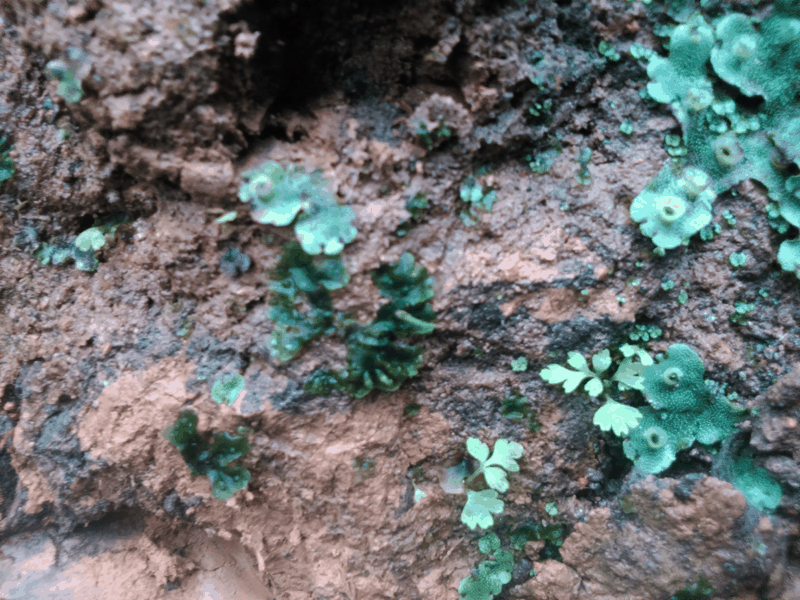
\includegraphics[width =
0.7\linewidth]
{biology-assets/botany-liverworts.png}
\end{figure}
Thalli of a marchantialean liverwort on a
wet earth bank, with young fern leaves;
photo from the 2014 field trip (Daniel's
field guide labels it ``Marchantiales with
receptacles'').

\section{Seedless vascular plants}
\label{section-pteridophytes}

Vascular plants with free-living
gametophytes and spores as the unit of
dispersal. The old group ``pteridophytes''
is not natural: living species form two
clades, the lycophytes and the monilophytes
(ferns and horsetails), the latter sister to
the seed plants \cite[Chapter
17]{evert2013raven}.

\begin{definition}
\label{definition-microphyll}
A \emph{microphyll} is a leaf with a single
vein whose trace leaves no gap in the stem
vascular cylinder; a \emph{megaphyll} has a
branched venation and a leaf gap.
\end{definition}

\begin{definition}
\label{definition-eusporangium}
A \emph{eusporangium} arises from several
surface cells, has a wall of several layers
and many spores; a \emph{leptosporangium}
arises from one cell, has a stalk, a wall
one cell thick with an annulus, and few
spores.
\end{definition}

\paragraph{Lycophytes} (microphylls,
eusporangia)
\cite[Chapter 17]{evert2013raven},
\cite[Chapter 11]{singh2010plant}:
\begin{itemize}
\item \emph{Lycopodiaceae} (club mosses:
\emph{Lycopodium}, \emph{Huperzia},
\emph{Lycopodiella}): leaves spiral, all
alike, without ligule; homosporous;
sporangia single on sporophylls, often in
strobili; spores trilete; gametophytes
either green or subterranean and
mycorrhizal, taking years to mature.
\item \emph{Selaginellaceae}
(\emph{Selaginella}): leaves with a small
ligule, often in four ranks of two sizes
(anisophyllous); rhizophores; heterosporous,
with endosporic gametophytes.
\item \emph{Isoetaceae} (\emph{Isoetes},
quillworts): ligulate, heterosporous, a corm
with a cambium; the last relatives of the
Carboniferous tree lycophytes.
\end{itemize}

\paragraph{Monilophytes}
\cite[Chapter 17]{evert2013raven},
\cite[Chapter 21]{stern2008introductory}:
\begin{itemize}
\item \emph{Psilotales}: \emph{Psilotum}
(whisk fern) has a dichotomously branched
aerial stem with tiny scales, no roots, a
rhizome with rhizoids, and sporangia fused
in threes (synangia); \emph{Tmesipteris}
has larger one-veined leaves and
synangia of two sporangia
\cite[Chapter 11]{singh2010plant}.
Gametophytes subterranean, with fungi.
\item \emph{Ophioglossales}
(\emph{Ophioglossum}, \emph{Botrychium}):
a leaf with a sterile blade and a fertile
spike with eusporangia.
\item \emph{Equisetum} (horsetails, about
15 species): ribbed jointed stems with
silica in the epidermis, whorls of small
scale leaves, a hollow pith, small
water-conducting carinal canals opposite the
ribs and larger air-filled vallecular canals
opposite the grooves; sporangia on
umbrella-shaped sporangiophores in apical
strobili; homosporous spores with elaters
(bands attached to the spore wall); green
free-living gametophytes. A genus almost
unchanged since the Carboniferous.
\item \emph{Marattiales}: large eusporangiate
ferns with sporangia often fused in
synangia.
\item \emph{Leptosporangiate ferns}
(Polypodiales and relatives, at least 10,500
species): circinate vernation (fiddleheads),
rhizomes, leptosporangia in sori on the
underside of the frond, with or without a
protective indusium; the annulus snaps the
sporangium open and catapults the spores.
\item \emph{Water ferns} (Salviniales), the
only living heterosporous ferns:
\emph{Marsilea}, with four-leaf-clover
leaves and drought-resistant sporocarps;
\emph{Azolla}, floating, with the
nitrogen-fixing cyanobacterium
\emph{Anabaena} in its leaves.
\end{itemize}

\section{Gymnosperms}
\label{section-gymnosperms}

Seed plants whose ovules are not enclosed in
a carpel. All are woody, with a bifacial
vascular cambium (secondary xylem inside,
secondary phloem outside).

\begin{definition}
\label{definition-ovule}
An \emph{ovule} is a megasporangium (the
nucellus) wrapped in an integument with an
opening, the micropyle; a single megaspore
survives inside and forms the female
gametophyte. A \emph{seed} is a ripened
ovule: embryo, stored food and seed coat
(from the integument).
\end{definition}

The oldest seeds are Late Devonian, about
365 million years old. The pollen grain is
the male gametophyte; it reaches the ovule
by wind or insects, so fertilization no
longer needs external water. Four living
phyla \cite[Chapter 18]{evert2013raven},
\cite[Chapter 12]{singh2010plant}:
\begin{itemize}
\item \emph{Coniferophyta} (about 630
species): needle or scale leaves with sunken
stomata and resin canals; dense wood of
tracheids with bordered pits; long and
short (spur) shoots; the ovulate cone is
compound, each unit an ovuliferous scale
bearing two ovules plus a sterile bract.
Examples from the field trip:
\emph{Pinus}, \emph{Abies religiosa}
(oyamel), \emph{Juniperus} (dioecious).
\item \emph{Cycadophyta} (11 genera, about
300 species): palm-like, once-pinnate
leaves, dioecious, cone-like strobili,
mostly insect-pollinated; a pollen tube
that releases large multiflagellated sperm
near the archegonia; seeds with a fleshy
outer coat.
\item \emph{Ginkgophyta}: \emph{Ginkgo
biloba} alone, deciduous fan-shaped leaves
on spur shoots, dioecious, swimming sperm,
fleshy-coated seeds.
\item \emph{Gnetophyta} (about 75 species):
\emph{Ephedra} (about 40 species, shrubs of
dry regions with scale leaves and jointed
green stems), \emph{Gnetum} (tropical trees
and lianas with broad leaves) and
\emph{Welwitschia mirabilis} (coastal desert
of southwestern Africa). Angiosperm-like
traits: vessels in the xylem, no archegonia
in \emph{Gnetum} and \emph{Welwitschia}, and
a double fertilization in \emph{Ephedra} and
\emph{Gnetum} whose second product is an
extra embryo that aborts, not an endosperm.
\end{itemize}

\paragraph{The pine life cycle}
\cite[Chapter 18]{evert2013raven}.
\begin{enumerate}
\item Pollen cones make winged pollen
grains (immature male gametophytes); in
spring they reach ovulate cones and stick to
pollination drops, which pull them through
the micropyle to the nucellus.
\item In each ovule one megaspore of four
survives; the female gametophyte develops
slowly, first as free nuclei.
\item The pollen tube grows slowly through
the nucellus; about 15 months after
pollination two or three archegonia are
ready and one sperm fertilizes the egg.
\item The embryo grows in the female
gametophyte tissue (the food of the seed);
the integument becomes the seed coat; seeds
are shed in the autumn of the second year.
\end{enumerate}

\begin{figure}[ht]
\centering
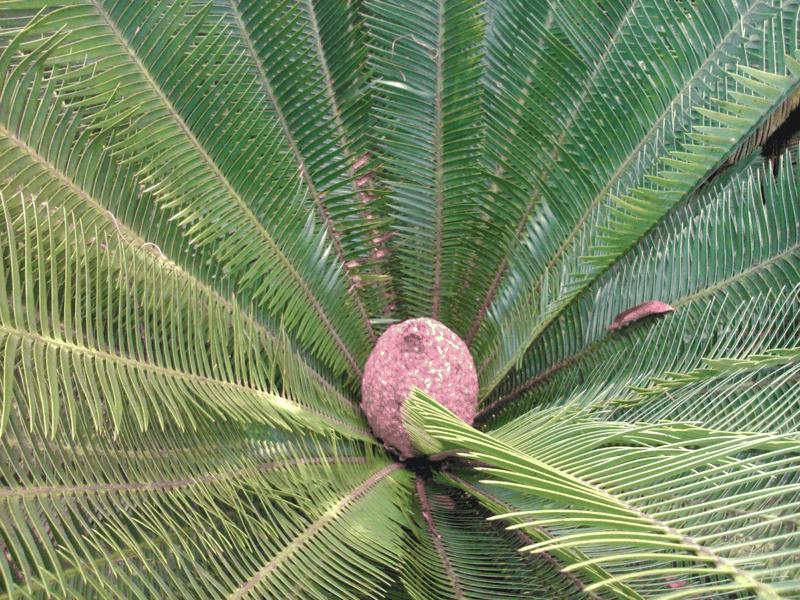
\includegraphics[width =
0.7\linewidth]
{biology-assets/botany-cycad.png}
\end{figure}
A cycad with a female strobilus in the
centre of its crown of pinnate leaves, at
the cycad nursery in Tlapacoyan, Veracruz,
visited in the 2014 field trip, where
\emph{Ceratozamia} and \emph{Dioon} were
grown (genus of this plant not recorded).

\section{Fossils and organ evolution}
\label{section-fossils}

\paragraph{Timeline}
\cite[Chapters 3--4]{willis2002evolution},
\cite[Chapters 17--18]{evert2013raven}.
\begin{center}
\begin{tabular}{ll}
Age & Event \\
\hline
Late Ordovician & spores in tetrads, \\
(about 450 Ma) & first land plants \\
Early Silurian & single trilete spores, \\
(about 430 Ma) & cuticle, tracheid-like \\
& tubes \\
Silurian & \emph{Cooksonia}, oldest \\
(about 428 Ma) & known vascular plant \\
Latest Silurian & stomata \\
(about 408 Ma) & \\
Early Devonian & Rhynie chert flora \\
(about 400 Ma) & (\emph{Rhynia}, \\
& \emph{Aglaophyton}) \\
Devonian & lycophytes, \\
& trimerophytes, first \\
& trees (\emph{Archaeopteris}) \\
Late Devonian & first seeds \\
(about 365 Ma) & \\
Carboniferous & coal swamps: tree \\
& lycophytes, \emph{Calamites}, \\
& tree ferns, seed ferns, \\
& cordaites \\
Permian--Mesozoic & seed plants dominate; \\
& cycads, ginkgos, \\
& Bennettitales, conifers \\
Early Cretaceous & \emph{Archaefructus}, \\
(about 125 Ma) & early angiosperm \\
\end{tabular}
\end{center}

Fossil groups the course asked about:
\begin{itemize}
\item \emph{Rhyniophytes} (\emph{Cooksonia},
\emph{Rhynia}): leafless, rootless,
dichotomous axes with terminal sporangia.
\item \emph{Zosterophyllophytes}
(\emph{Zosterophyllum}): lateral
kidney-shaped sporangia; the line leading
to lycophytes.
\item \emph{Trimerophytes}
(\emph{Psilophyton}): a main axis with
smaller side branches; the line leading to
ferns, horsetails and seed plants.
\item Carboniferous trees:
\emph{Lepidodendron} (tree lycophyte,
heterosporous, cones at branch tips) and
\emph{Calamites} (tree horsetail with
secondary xylem).
\item \emph{Progymnosperms}
(\emph{Archaeopteris}, wood called
\emph{Callixylon}): conifer-like wood and
a bifacial cambium, but reproduction by
spores; the likely precursors of seed
plants.
\item Seed ferns (e.g.\ medullosans):
fern-like leaves bearing seeds, at the base
of seed-plant phylogeny; cordaites, early
conifer-like trees; Bennettitales and
Caytoniales, Mesozoic groups proposed as
relatives of the angiosperms.
\end{itemize}

\paragraph{Theories of organ evolution.}
\begin{itemize}
\item \emph{Telome theory} (Zimmermann,
1952): the first plants were dichotomous
axes whose terminal branches are telomes.
Elementary processes: overtopping (one
branch becomes the main axis), planation
(branches come to lie in one plane),
webbing (tissue fills the space between
them) and reduction. Overtopping, planation
and webbing make a megaphyll; reduction
can make a microphyll. Fusion of sterile
telomes around a megasporangium is the
proposed origin of the integument, seen in
the free lobes of early seeds such as
\emph{Elkinsia} \cite[Chapter
4]{willis2002evolution},
\cite[Chapters 17--18]{evert2013raven}.
\item \emph{Enation theory} (Bower, 1935):
microphylls began as unvascularized
outgrowths of the stem (enations), as on
\emph{Sawdonia}, into which a vascular trace
later extended.
\item \emph{Lignier}: the aerial and
underground parts of an alga-like ancestral
axis became stem and root.
\item \emph{Stelar theory}: the vascular
cylinder evolved from a solid central
protostele to the siphonostele (with pith)
and the eustele (separate strands around a
pith) of seed plants.
\end{itemize}
Life-cycle trend, from the course notes and
\cite[Chapter 4]{willis2002evolution}:
homospory, then heterospory (shown by two
size classes of dispersed spores rising
through the Devonian), then abortion of
three of the four megaspores, then the
seed. Heterospory keeps the vulnerable
gametophyte short-lived and protected.

\section{The plant cell and plant tissues}
\label{section-tissues}

\paragraph{The plant cell}
\cite[Chapter 3]{evert2013raven}. Besides
the usual eukaryotic organelles, plant
cells have a cellulose cell wall, a large
central vacuole, and plastids. Every
plastid has an envelope of two membranes;
the main kinds are chloroplasts
(photosynthesis), chromoplasts (yellow to
red pigments, in petals and fruits) and
leucoplasts, among them amyloplasts (starch)
and elaioplasts (oil). Inside a chloroplast
are the stroma and the thylakoids, flattened
sacs that are stacked in grana and joined by
unstacked stroma thylakoids (lamellae).
Chloroplasts keep traits of their bacterial
ancestors: several copies of a circular DNA
without histones, small ribosomes, and
division by binary fission.

\paragraph{Meristems.}
Primary growth (in length) comes from the
apical meristems of shoot and root, whose
products, the primary meristems protoderm,
ground meristem and procambium, give the
three tissue systems. Secondary growth (in
thickness) comes from the lateral
meristems: the vascular cambium, and the
cork cambium (phellogen), which makes the
periderm: cork outside, phelloderm inside
\cite[Chapters 23, 26]{evert2013raven}.

\begin{center}
\begin{tabular}{lll}
System & From & Tissues \\
\hline
Dermal & protoderm & epidermis \\
& & (stomata, \\
& & trichomes); \\
& & later periderm \\
Ground & ground & parenchyma, \\
& meristem & collenchyma, \\
& & sclerenchyma \\
Vascular & procambium & xylem, phloem \\
\end{tabular}
\end{center}

\paragraph{Cell types}
\cite[Chapter 23]{evert2013raven}.
\begin{itemize}
\item \emph{Parenchyma}: living, thin
walled, the most common; photosynthesis
(mesophyll), storage of starch, oil or
water, secretion.
\item \emph{Collenchyma}: living, with
unevenly thickened walls; support of
growing stems and leaves.
\item \emph{Sclerenchyma}: thick lignified
secondary walls, often dead at maturity;
long fibers and short sclereids (e.g.\ the
stone cells of the pear).
\item \emph{Xylem}: tracheids and, in most
angiosperms, vessel elements, whose end
walls have perforations; both are dead
when functional.
\item \emph{Phloem}: sieve cells
(gymnosperms) or sieve-tube elements with
sieve plates and companion cells
(angiosperms).
\item \emph{Epidermis}: a layer covered by
the cuticle, with guard cells around the
stomata and hair-like trichomes.
\end{itemize}

\section{Photosynthesis}
\label{section-photosynthesis}

This rests on Daniel's exam notes from
Biolog\'ia de Plantas II, checked against
\cite[Chapter 7]{evert2013raven}.
$$
\mathrm{6\,CO_2 + 6\,H_2O
\rightarrow C_6H_{12}O_6 + 6\,O_2}
$$

\paragraph{Pigments.}
Chlorophyll $a$ turns light into chemical
energy; chlorophyll $b$ and carotenoids are
accessory, and carotenoids also protect the
apparatus from photo-oxidation;
phycobilins play the accessory role in
cyanobacteria and red algae. An excited
pigment can re-emit the photon, pass the
energy to a neighbour by resonance, or pass
an electron to an acceptor; antenna
complexes funnel energy to reaction centres.

\paragraph{Light reactions} (thylakoid
membranes). Two photosystems in series,
drawn by redox potential as the
\emph{Z scheme}:
\begin{enumerate}
\item Photosystem II (reaction centre P680)
gives an electron to pheophytin and then to
plastoquinones $Q_A$ and $Q_B$; its
water-splitting complex replaces the
electron and releases $\mathrm{O_2}$ and
protons into the lumen.
$$
\mathrm{2\,H_2O \rightarrow
O_2 + 4\,H^+ + 4\,e^-}
$$
\item Plastoquinol carries the electrons to
the cytochrome $b_6f$ complex, releasing
into the lumen the protons it took up from
the stroma; plastocyanin then carries the
electrons to Photosystem I.
\item Photosystem I (P700), excited again,
passes the electrons through ferredoxin to
ferredoxin-NADP$^+$ reductase, which
reduces $\mathrm{NADP^+}$ to NADPH in the
stroma.
\item The proton gradient drives ATP
synthase (chemiosmosis), as in
mitochondria.
\end{enumerate}
In \emph{cyclic} electron flow ferredoxin
returns electrons to the cytochrome
$b_6f$ complex: ATP is made without NADPH.

\paragraph{Calvin cycle} (stroma), three
stages:
\begin{enumerate}
\item fixation: rubisco adds $\mathrm{CO_2}$
to ribulose 1,5-bisphosphate (RuBP); the
six-carbon product splits into two
3-phosphoglycerate (PGA);
\item reduction: PGA is phosphorylated by
ATP and reduced by NADPH to
glyceraldehyde 3-phosphate (PGAL);
\item regeneration: five of every six PGAL
rebuild RuBP, using more ATP.
\end{enumerate}
Three turns fix three $\mathrm{CO_2}$ into
one net PGAL at a cost of 9 ATP and 6
NADPH. PGAL leaves the chloroplast to make
sucrose, or stays and becomes starch.

\paragraph{Photorespiration.}
Rubisco also takes $\mathrm{O_2}$: RuBP
plus $\mathrm{O_2}$ gives one PGA and one
two-carbon phosphoglycolate, which the
Calvin cycle cannot use. A salvage pathway
through chloroplast, peroxisome and
mitochondrion turns two glycolates into
serine plus $\mathrm{CO_2}$ and returns 75\%
of the carbon as PGA, spending ATP and
reducing power. It increases when stomata
close and $\mathrm{O_2}$ builds up relative
to $\mathrm{CO_2}$ inside the leaf.

\paragraph{C4 plants} (Hatch--Slack
pathway). In mesophyll cells PEP
carboxylase, which uses bicarbonate and
ignores $\mathrm{O_2}$, adds it to
phosphoenolpyruvate (PEP), giving the
four-carbon oxaloacetate, then malate (or
aspartate). This moves into the
bundle-sheath cells (Kranz anatomy, a
wreath of sheath cells around each vein),
where it releases $\mathrm{CO_2}$ to rubisco
and the Calvin cycle; pyruvate returns and is
turned back into PEP with ATP. Pumping
$\mathrm{CO_2}$ into the sheath suppresses
photorespiration, and C4 plants
photosynthesize
with narrower stomata and less water loss.

\paragraph{CAM plants} (crassulacean acid
metabolism; cacti, stonecrops, agaves).
Stomata open at night: PEP carboxylase fixes
$\mathrm{CO_2}$ into oxaloacetate and
malate, stored as malic acid in the large
vacuole. By day stomata close; malate is
decarboxylated and the $\mathrm{CO_2}$
enters the Calvin cycle in the same cell.
C4 separates the two carboxylations in
space, CAM in time. A CAM plant loses 50--100
g of water per gram of $\mathrm{CO_2}$
fixed, against 250--300 g for C4 and
400--500 g for C3 plants.

\section{Angiosperms and Agavaceae}
\label{section-angiosperms}

This section is written from the textbooks;
the surviving coursework has no material on
it.

Angiosperms (phylum Anthophyta) are seed
plants whose ovules are enclosed in a
carpel, which becomes the fruit wall; the
oldest well-known fossil,
\emph{Archaefructus}, is about 125 million
years old \cite[Chapters
19--20]{evert2013raven}.

\paragraph{The flower}
\cite[Chapter 19]{evert2013raven}. Four
whorls on the receptacle, from outside in:
\begin{itemize}
\item sepals (together the calyx) and
petals (the corolla), the sterile perianth;
when alike they are called tepals;
\item stamens (the androecium):
microsporophylls, each a filament with an
anther where pollen forms;
\item carpels (the gynoecium):
megasporophylls folded around the ovules,
each with ovary, style and stigma; a single
carpel or several fused carpels is a
pistil.
\end{itemize}
The ovary is \emph{superior} if the other
parts attach below it and \emph{inferior}
if they attach above it. Flowers with
stamens and carpels are perfect; a species
with separate male and female flowers on
one plant is monoecious, on different
plants dioecious. The female gametophyte
(embryo sac) usually has seven cells and
eight nuclei; in double fertilization one
sperm fertilizes the egg and the other
fuses with the two polar nuclei, giving the
triploid endosperm.

\paragraph{Monocots and eudicots.}
The old ``dicots'' are not a natural
group: the eudicots are a clade, and a few
early lineages (e.g.\ \emph{Amborella}, the
magnoliids) are neither monocots nor
eudicots. Main differences
\cite[Table 19-1]{evert2013raven}:
\begin{center}
\begin{tabular}{lll}
& Monocots & Eudicots \\
\hline
Flower parts & in threes & in fours \\
& & or fives \\
Pollen & one aperture & three \\
& & apertures \\
Cotyledons & one & two \\
Leaf veins & parallel & netlike \\
Stem bundles & scattered & in a ring \\
Secondary & rare & common \\
growth & & \\
\end{tabular}
\end{center}
Monocots have at least 90,000 species,
eudicots at least 200,000. Merosity is the
quickest field test: a lily has three
sepals, three petals, six stamens and three
fused carpels; a typical eudicot flower has
parts in fives or fours. Both columns say
``usually'': the cacti below are eudicots
with numerous spiral flower parts.

\paragraph{Agavaceae}
\cite[Chapter 7]{simpson2006plant}. A
monocot family (order Asparagales) of about
8--12 genera and over 300 species, from the
central United States to northern South
America: rosettes of large fibrous,
parallel-veined, often spiny leaves, on a
short stem or a trunk. Flowers trimerous:
3+3 tepals, 6 stamens, 3 fused carpels with
a superior or inferior ovary, septal
nectaries; fruit a capsule or
indehiscent; black
flattened seeds. A distinctive karyotype of
5 long and 25 short chromosomes. Many grow
in dry places and have CAM. Uses: fibres
(sisal from \emph{Agave sisalana},
henequen from \emph{A. fourcroydes}), food,
soap, and tequila from \emph{A. tequilana};
\emph{Yucca} is pollinated by yucca moths
that lay eggs in its ovary.

\section{Cactaceae}
\label{section-cactaceae}

The second course handed out the Cactaceae
fascicle of the \emph{Flora del Valle de
Tehuac\'an-Cuicatl\'an}
\cite{arias2012cactaceae}, a published
regional flora with keys and descriptions
of 28 genera. From it, with
\cite[Chapter 8]{simpson2006plant}:

\paragraph{The family.}
Eudicots of the order Caryophyllales.
Mostly stem succulents, leaves vestigial
or absent (well developed in
\emph{Pereskia}). The spines grow from
areoles, specialized axillary short shoots
covered with hairs, which also produce new
stems and flowers. Flowers usually
solitary, bisexual, with many spirally
arranged tepals grading from bract-like to
petal-like, many stamens, and an inferior
ovary of three to many carpels with one
locule and many ovules; the fruit is
usually a berry. Betalain pigments instead
of anthocyanins. Photosynthesis is CAM
(Section~\ref{section-photosynthesis}),
which fits the succulent, water-storing
stem.

\begin{definition}
\label{definition-areole}
An \emph{areole} is a specialized
axillary meristem of a cactus, covered with
hairs, from which the spines (modified
leaves), new branches and flowers arise.
\emph{Glochids} are small hair-like
leaves with backward barbs on the areoles
of Opuntioideae.
\end{definition}

\paragraph{Numbers}
\cite[pp.~2--3]{arias2012cactaceae}.
About 126 genera and 1900 species
(Anderson) or 124 genera and 1438 species
(Hunt). Mexico has 60 genera and 670
species, 77\% endemic. The
Tehuac\'an-Cuicatl\'an Valley has 28
genera and 86 species, 21 of them endemic
to the region and 5 introduced. The family
is native to the Americas; only
\emph{Rhipsalis} also reaches Africa,
Madagascar and Sri Lanka, and some
\emph{Opuntia} are naturalized in the Old
World and Australia.

\paragraph{Subfamilies.}
Four: Pereskioideae (paraphyletic, leafy),
Maihuenioideae, Opuntioideae and
Cactoideae. Only the last two occur in the
valley, separated by the flora's key:
\begin{itemize}
\item areoles without glochids, seeds brown
to black without aril: Cactoideae
(columnar, barrel and globose cacti:
\emph{Cephalocereus}, \emph{Pachycereus},
\emph{Stenocereus}, \emph{Ferocactus},
\emph{Mammillaria} and others);
\item areoles with glochids, seeds pale
with an aril: Opuntioideae (\emph{Opuntia},
\emph{Cylindropuntia},
\emph{Pereskiopsis}).
\end{itemize}

\paragraph{Uses recorded in the flora.}
\emph{Acanthocereus subinermis} (``nopal
de cruz''): young stems eaten cooked and
used as living fences. \emph{Hylocereus
undatus} (``pitahaya''): edible fruit.
\emph{Myrtillocactus geometrizans}
(``garambullo''): fruit eaten fresh. Several
columnar cacti serve as living fences and
for fruit eaten fresh or as \emph{agua
fresca}. Nopales and prickly pears
(\emph{Opuntia}) are the best-known food
cacti \cite[Chapter 8]{simpson2006plant}.

\section{Field trip and ethnobotany}
\label{section-field-trip}

\paragraph{The field trip, 24--26 October
2014.} From Mexico City across Puebla to
Tlapacoyan, Veracruz, and back, sampling
bryophytes, pteridophytes and gymnosperms
along an altitudinal transect; specimens
were identified each evening for a
microherbarium. Daniel's group wrote it up
as a field guide in LaTeX, with an
itinerary, site descriptions and a photo
record.
\begin{center}
\begin{tabular}{lll}
Site & m & Collected \\
\hline
Llano Grande & 3223 & \emph{Pinus}, \\
(conifer & & \emph{Abies religiosa}, \\
forest) & & moss with \\
& & sporophyte \\
El Ocotal & 2342 & \emph{Juniperus}, \\
(pine-oak) & & \emph{Pinus cembroides}, \\
& & \emph{Selaginella} \\
R\'io Alseseca & 1210 & \emph{Anthoceros}, \\
(cloud & & \emph{Marchantia}, \\
forest) & & \emph{Marattia}, \\
& & \emph{Equisetum}, \\
& & tree fern, \\
& & \emph{Huperzia} \\
La Tomata & 530 & \emph{Lycopodium}, \\
(tropical & & epiphytic \\
forest) & & \emph{Psilotum}, \\
& & Polytrichales \\
R\'io Filobobos & 280 & ferns, \\
(rainforest) & & \emph{Equisetum} \\
Zoatzingo & 2100 & \emph{Botrychium} \\
Alchichica & 2350 & \emph{Ephedra} \\
(xeric scrub) & & \\
\end{tabular}
\end{center}
The group also visited a cycad nursery in
Tlapacoyan with \emph{Ceratozamia} and
\emph{Dioon} from seed to cone-bearing
adults. The transect runs from temperate
conifer forest through cloud forest, where
bryophytes and ferns were richest, to
lowland tropical forest, and back up to the
dry scrub of the Alchichica basin, where
the only plant collected was the
desert gymnosperm \emph{Ephedra}.

\paragraph{Ethnobotany of \emph{Equisetum}.}
Ethnobotany studies the relations between
people and plants; John Harshberger used the
word in 1895 \cite[Chapter
1]{young2007ethnobotany}. For the course,
Daniel's group interviewed a vendor at the
Xochimilco plant market about
\emph{Equisetum}. Common names: ``cola de
caballo'', ``carricillo'', ``carrizo'',
``ca\~na de los \'angeles''. Uses:
ornamental; polishing soft metals, thanks
to the silica in the epidermis; and
medicinal, mainly for digestive, liver,
gallstone, urinary, menstrual and skin
complaints. The plants come from collectors
in Veracruz, Puebla, the Estado de M\'exico
and Hidalgo.

\bibliography{my}
\bibliographystyle{amsalpha}

\end{document}
